\chapter{Theoretical Background}

% talk about cold water patches here. What are they, why are they interesting? Especially with respect to the salmanoid fish stuff. How are they defined. What is the critigue about the definition


\section{Model Input Sensitivity Analysis}

The inputs to models can diver and are generally dependent in their structure and manyfoldness on the nature of the model itself. Under the light of sensitivity analysis however, it can be worthwhile to define, what the inputs to a model actually contains. In sensitivity analysis, everything that causes variation in the output of the model is classified as an input \citep{saltelli_global_2007}. Providing an example: If a linear regression of a target variable $Y$ is performed, then not only are the predictors $X_1, \dots, X_n$ considered as model inputs, but also the parameters $\theta_1, \dots, \theta_n$ that correspond to the predictors. So the model:

\begin{equation}
	Y = f(X_1, X_2, \theta_1, \theta_2)
	\label{eq:model_with_params}
\end{equation}

would have four parameters from the view of sensitivity analysis. 



\section{Sensitivity Analysis}

According to Saltelli et al. sensitivity analysis is ``The study of how uncertainty in the output of a model [\dots] can be apportioned to different sources of uncertainty in the model input'' \citep{saltelli_sensitivity_2004}. Sensitivity analysis provides a range of benefits. Firstly it allows the modeller to apply a strategy called ``Factor Fixing'': if the model output $Y$ is found to be independent of one or multiple parameters $\theta_i$, then these can be set to fixed constants. It may then even be possible to condense a complete submodule of a model if all parameters connected to that submodule are noninfluential, making sensitivity analysis a tool for model simplification \citep{saltelli_global_2007}. Secondly, sensitivity analysis generally improves model validity by identifying highly influential and therefore critical model components \citep{ligmann-zielinska_spatially-explicit_2013}.

\subsection{The Morris Method}

% also add to the morris method, that it is generally a method for models with an one dimensional output. Therefore when applied to models with multidimensional output, generally some spatial lumping into a scalar value has to be performed

The Morris method belongs to the group of screening methods in sensitivity analysis. These are ideal to filter a short list of important input parameters from computationally expensive models with a great number of input parameters. This can be done as these methods only require a relatively small number of model evaluations to provide sensitivity measures for the input parameters, making them a good choice when the target of the sensitivity analysis is Factor Fixing \citep{saltelli_global_2007}. As a global method, Morris explores the entire input space by varying all input parameters simultaneously across their plausible ranges, meaning that sensitivity scores reflect average behaviour across the full parameter space rather than being tied to a single point \citep{saltelli_how_2010}. The following explanation of the Morris method closely follows \citep{saltelli_global_2007} and is explained more explicitly in chapter 3 of their book.

\subsubsection{Elementary Effects and the Sampling Grid}

At the core of this introduction sits a $k$-dimensional model $Y$ with inputs $X_1, \dots, X_k$. These inputs all together can also be written in a vector $\mathbf{X}$. The model inputs are defined in the $k$-dimensional unit cube, meaning that $X_i$ can take on a value in the interval $[0,1]$. It is worth pointing out, that every model with a continuous input can be scaled to the $[0,1]$ range, which makes the unit cube a great place to define methods. In the Morris method, this input space is discretized into a grid $\Omega$. This grid features $p$ levels. 

An elementary effect of the $i$th input parameter $X_i$ is then defined as:

\begin{equation}
	EE_i = \frac{Y(X_1, X_2, \dots, X_{i-1}, X_i + \Delta, \dots, X_k) - Y(X_1, X_2, \dots, X_k)}{\Delta}
\end{equation}

Where $\Delta$ represents some step in the unit cube. $\Delta$ can be chosen from a range of different values, which are given by the set $\left\{\frac{1}{p-1}, \dots, 1 - \frac{1}{p-1}\right\}$.

\begin{figure}[h]
	\centering
	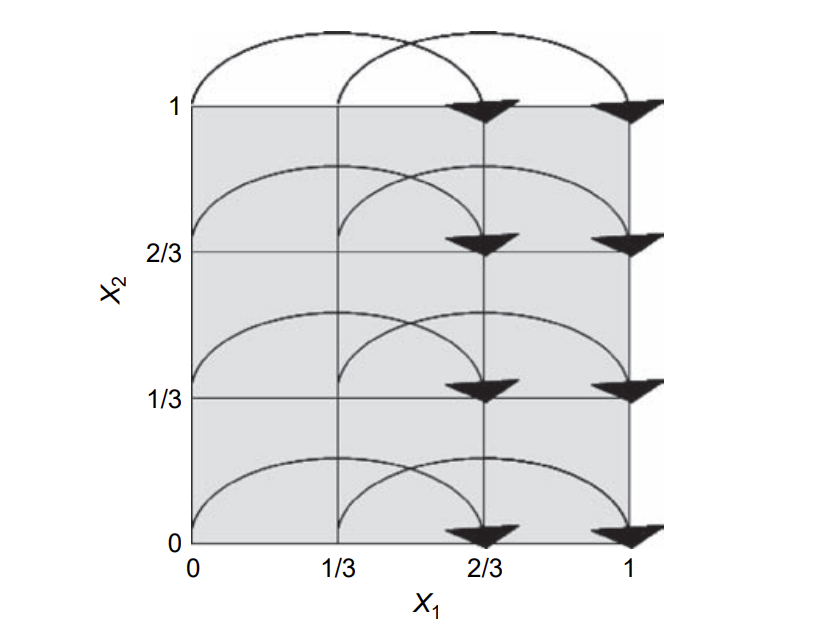
\includegraphics[width=0.7\textwidth]{Bilder/morris_grid.png}
	\caption{An example grid $\Omega$. The grid features two parameters $X_1$, $X_2$, meaning that it is a two-dimensional grid. Further, it features four levels ($p = 4$). The step length $\Delta$ chosen here is $\frac{2}{3}$, which corresponds to an element of the set of viable values for $\Delta$: $1 - \frac{1}{4-1} = 1 - \frac{1}{3} = \frac{2}{3}$.}
	\label{fig:morris_grid}
\end{figure}

In the definition of the elementary effect, the vector $\mathbf{X} = (X_1, X_2, \dots, X_k)$ has to fulfil the condition that $\mathbf{X} + \mathbf{e}_i \cdot \Delta$ still has to lie within the grid $\Omega$. $\mathbf{e}_i$ is a vector of zeros except having a one at its $i$th entry. So for instance:

\begin{equation}
	\mathbf{e}_2 = (0, 1, 0, \dots, 0)
\end{equation}

The Morris method occupies itself with finding the statistical distribution of each of the $i$ elementary effects. $\mathcal{F}_i$ is thereby used to denote the distribution of $EE_i$, in other words $\mathcal{F}_i \sim EE_i$ \citep{saltelli_global_2007}.

\subsubsection{Trajectory-Based Sampling}

To populate $\mathcal{F}_i$ with multiple samples of $EE_i$, the Morris method uses an efficient trajectory-based sampling design that obtains as many elementary effects as possible from as few model evaluations as possible.

The exact mathematical formulation of how trajectories are constructed is beyond the scope of this thesis; a visual understanding is sufficient. Figure~\ref{fig:saltelli_trajectory_grid}, taken from \citep{saltelli_global_2007}, shows an example trajectory through a three-dimensional sampling grid.

\begin{figure}[H]
	\centering
	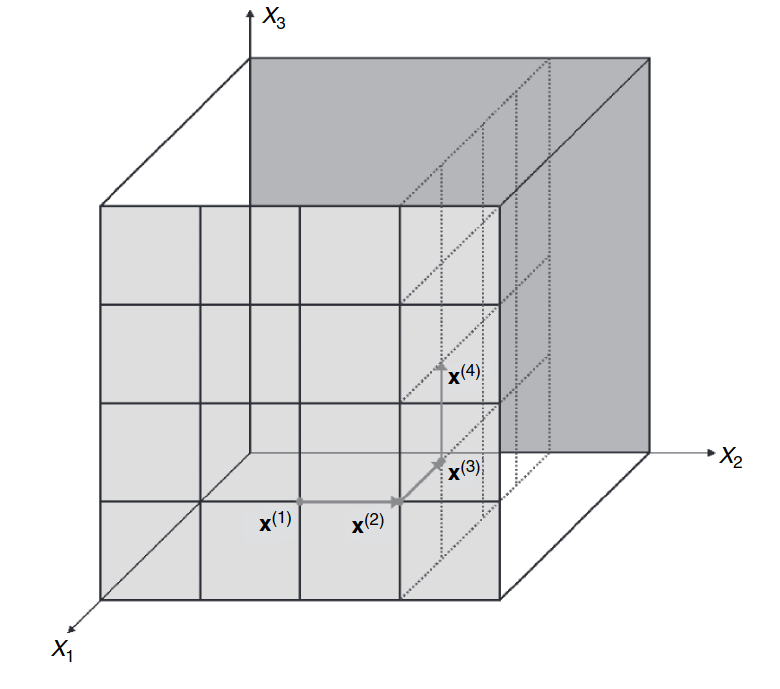
\includegraphics[width=0.7\textwidth]{Bilder/satteli_trajectory_grid.png}
	\caption{An example Morris trajectory through a three-dimensional sampling grid ($k = 3$, $p = 6$). The trajectory consists of $k+1 = 4$ points, with each consecutive pair of points differing in exactly one parameter. Reproduced from \citet{saltelli_global_2007}.}
	\label{fig:saltelli_trajectory_grid}
\end{figure}

From this figure it becomes visible that a trajectory consists of $k+1$ points $\mathbf{x}^{(1)}, \mathbf{x}^{(2)}, \dots, \mathbf{x}^{(k+1)}$, where $k$ is the dimension of the sampling grid. Each point differs from its predecessor by a step of $\Delta$ in exactly one grid direction, so that consecutive points differ in only one parameter. The trajectory is constructed such that each dimension of the grid is stepped along exactly once. Note that since the grid shown is three-dimensional ($k = 3$, matching the three parameters varied in this work), each trajectory consists of $k+1 = 4$ points.



Each trajectory yields exactly k elementary effects $EE_i$, one for each parameter spanning the sampling grid. A single trajectorybrequires $k+1$ model evaluations -- one at each point -- and yields exactly $k$ elementary effects: one estimate for each factor.

To build up $\mathcal{F}_i$ for every factor, $r$ such trajectories are generated. Since each trajectory contributes exactly one elementary effect per factor, each $\mathcal{F}_i$ ends up containing $r$ samples. The total number of model evaluations required is:




\begin{equation}
	N = r \cdot (k+1)
	\label{eq:morris_runs}
\end{equation}


\citep{saltelli_global_2007}.

\subsubsection{Choosing $\Delta$ and $r$}

% TODO: add the r choice

The choice of $p$ and $\Delta$ are not independent. When $p$ is chosen to be even, the choice $\Delta = \frac{p/2}{p-1}$ has the additional property of guaranteeing equal-probability sampling from the grid, meaning that all grid levels are sampled with equal probability across the $r$ trajectories \citep{saltelli_global_2007}.

\subsubsection{Sensitivity Measures: $\mu$, $\sigma$, and $\mu^*$}

Once the distributions $\mathcal{F}_i$ have been mapped out, statistical measures can be computed just like over every other statistical distribution. In Morris, the mean $\mu_i$ and the standard deviation $\sigma_i$ of $\mathcal{F}_i$ are computed. These two statistical measures together already allow for reasonable insight into the influence of the $i$th parameter $X_i$ which corresponds to the $i$th elementary effect $EE_i$:

If $\mu_i$ deviates strongly from $0$, then this means that the elementary effect $EE_i$ generally takes on non-zero values and therefore that the model output changes notably when a step of $\Delta$ is performed along the dimension spanned by $X_i$. This then ultimately means, that changes in $X_i$ seem to generally affect the model output $Y$ considerably and $X_i$ therefore receives a high sensitivity score. Generally, the more $\mu_i$ deviates from zero, the larger the sensitivity of the model output towards $X_i$.

If $\sigma_i$ is large, this means that the distribution $\mathcal{F}_i$ is spread out considerably over a larger range. This indicates, that the elementary effects $EE_i$ that were computed were generally different depending on their location in the grid. Meaning that in one area, the model might only yield small changes in output, when $X_i$ is varied while in other areas $X_i$ leads to strong changes in model output. This behaviour points either to nonlinearity regarding $X_i$ or to the fact that $X_i$ interacts with other input parameters. Which effect is responsible for the high standard deviation (or whether both are responsible for the effect at the same time) can not be determined. Which is a shortcoming of the method of Morris \citep{saltelli_global_2007}. Figure \ref{fig:mu_sig_example} provides an visual example of possible F distributions of a Factor $X_i$ with the associated $\mu$ and $\sigma$ values and the corresponding interpretation.

\begin{figure}[H]
	\centering
	
\includegraphics[width=1\textwidth]{Bilder/example_grid_mu_sigma_vairation.png}
	\caption{Different F distributions of a parameter $X_i$ are shown. Additionally, $\mu$ and $\sigma$ of each distribution is provided. An interpetation is provided}
	\label{fig:mu_sig_example}
\end{figure}

Situations can occur, where $\mathcal{F}_i$ contains many extreme values however the distribution is symmetric around zero. One such example is visualized in \ref{fig:mu_sig_example} in the upper left plot. In such cases computing the mean value $\mu_i$ will yield a value close to zero and we would assume, that the parameter $X_i$ therefore is noninfluential. This would be a faulty assumption, as the sampled elementary effects $EE_i$ are substantial in their magnitude but just cancel themselves out. This phenomenon can be spotted by always taking $\sigma_i$ into consideration, as in this scenario $\sigma_i$ is large, but it is more common to also sample an additional distribution $\mathcal{G}_i$ which captures the magnitude of the elementary effects $|EE_i|$. So $\mathcal{G}_i \sim |EE_i|$. We then compute the mean of this distribution $\mu^*_i$ which can be interpreted like $\mu_i$. The further away from zero, the more influential is the parameter. But since it is the magnitude, the distribution never features negative values and therefore cancellation effects can not occur \citep{saltelli_global_2007}. Figure \ref{fig:mu_mu_star} provides a visual example for this phenomenon.

\begin{figure}[H]
	\centering
	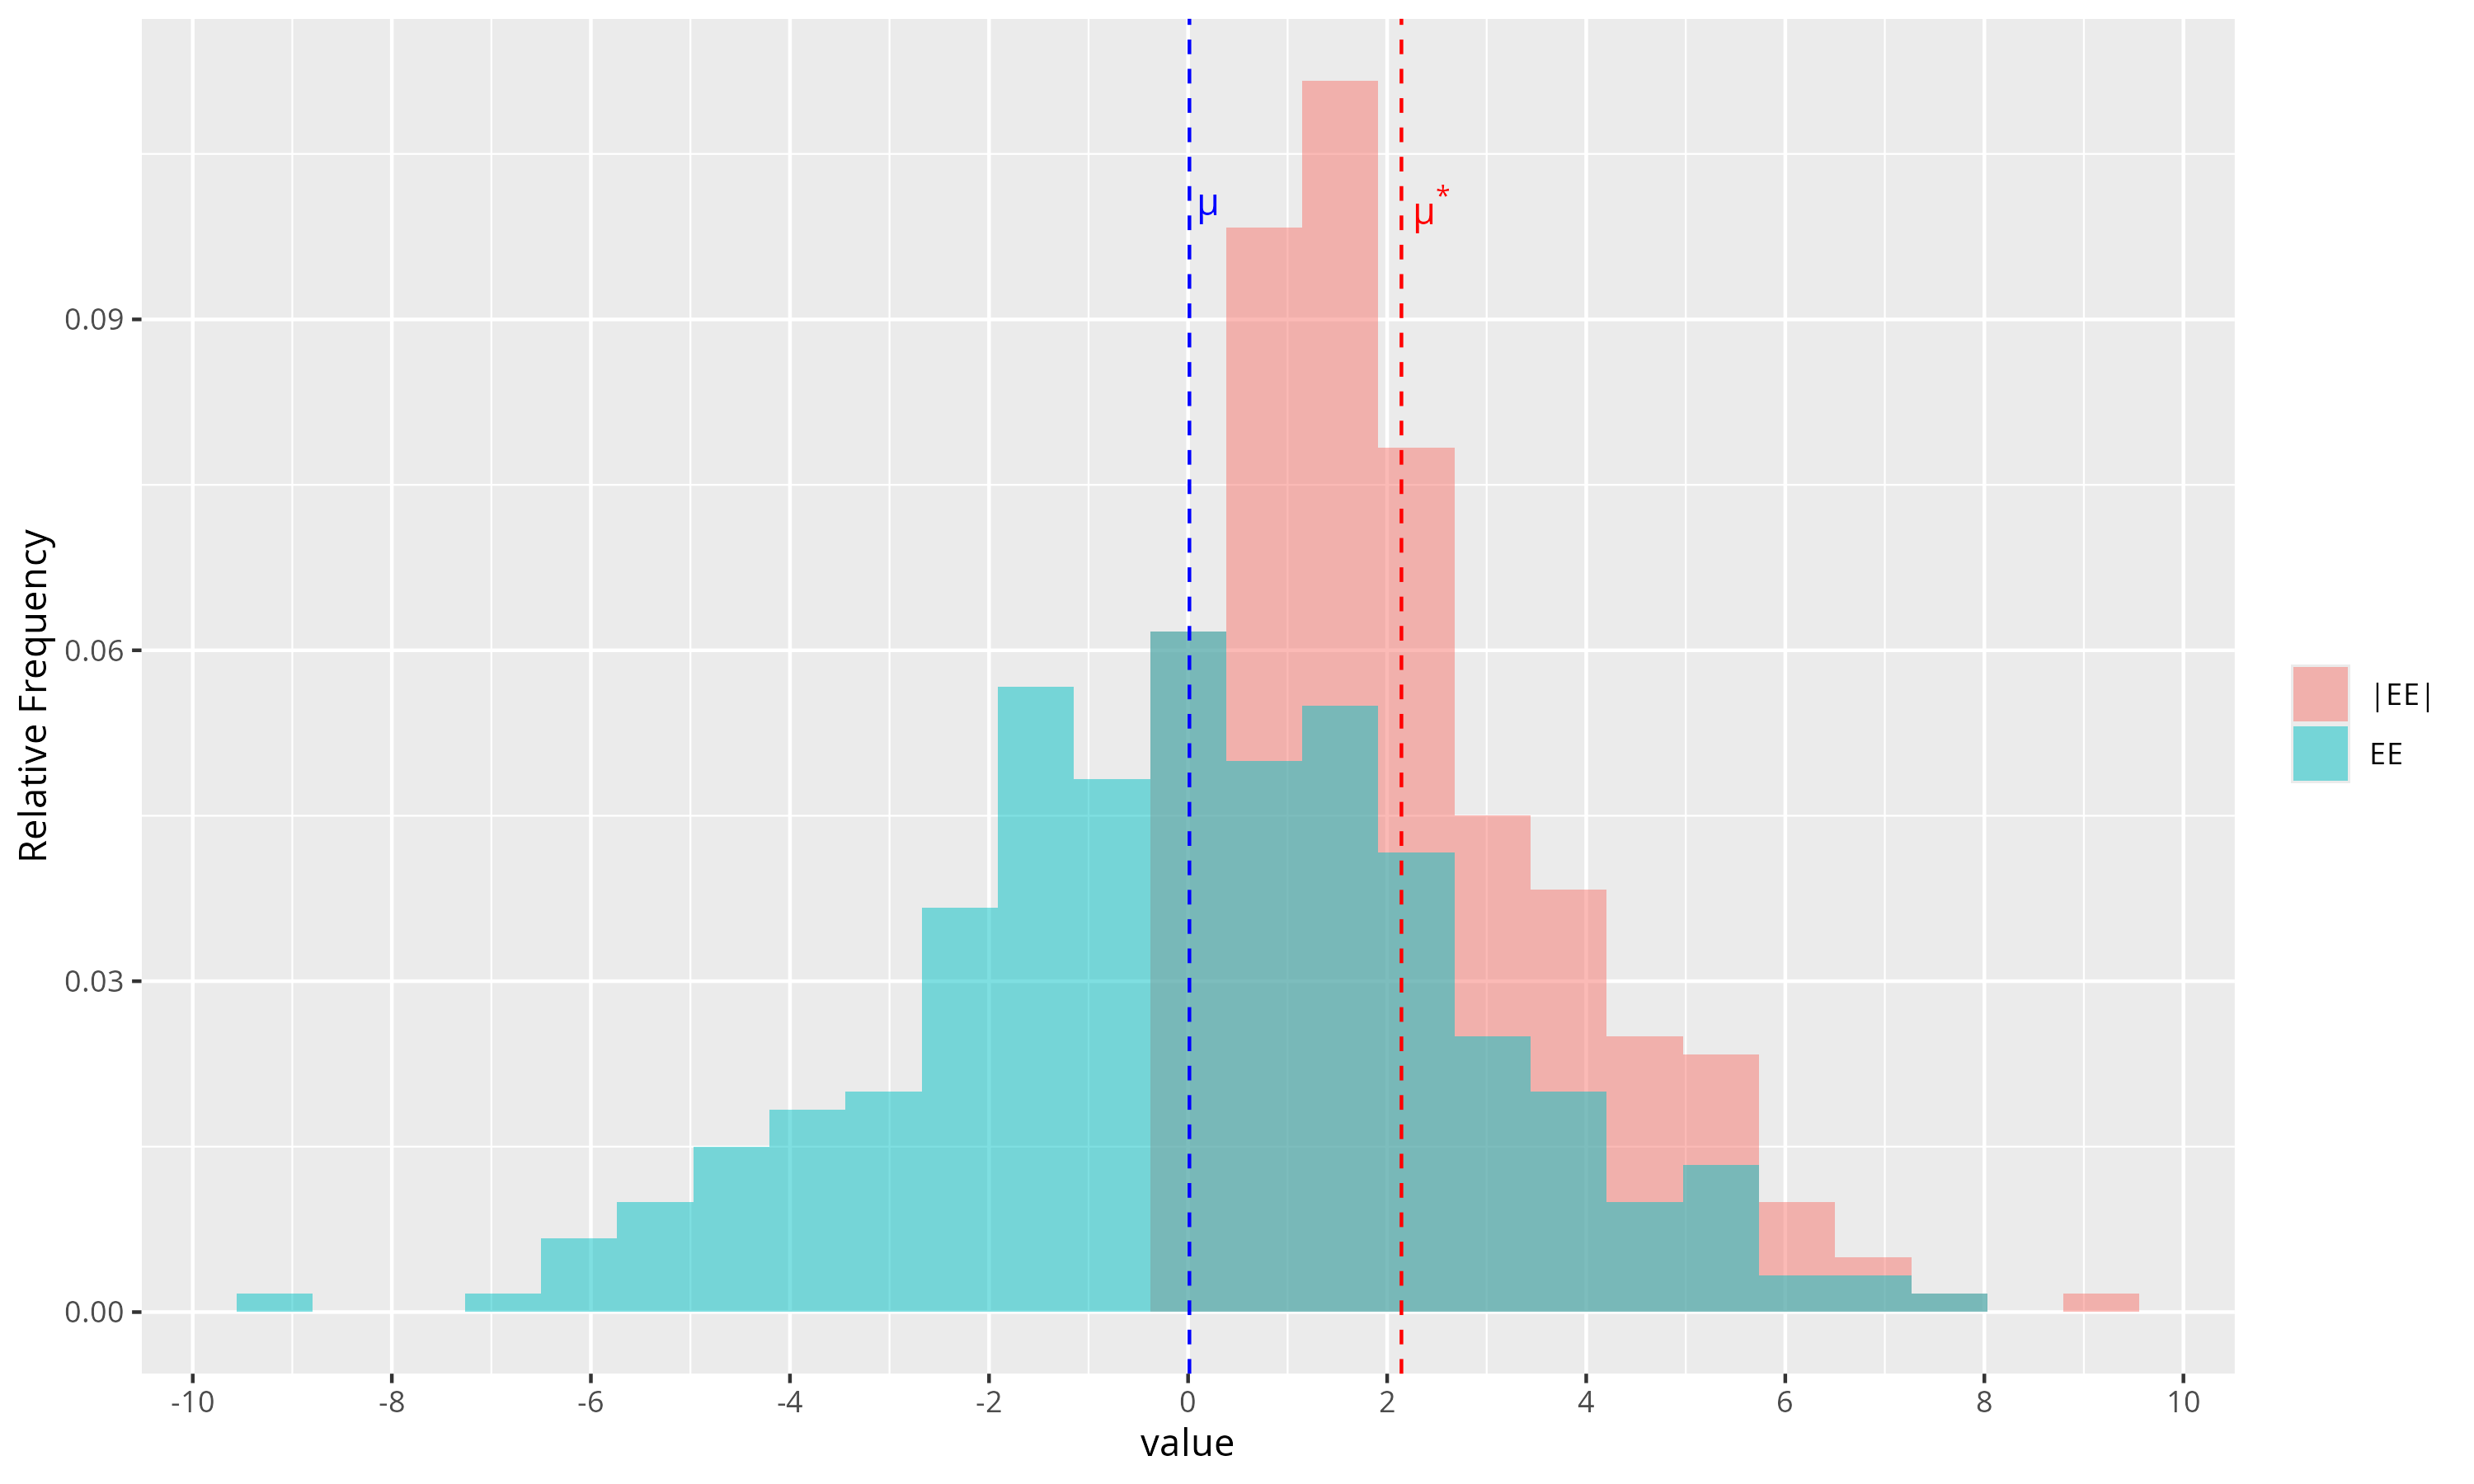
\includegraphics[width=1\textwidth]{Bilder/mu_mu_star.png}
	\caption{The difference of $\mu$ and c visualized with their underlying distribution $\mathcal{G}$ and $\mathcal{F}$. While the mean $\mu$ of the distributuion $\mathcal{F}$ lies at around zero, $\mu^{\star}$ significantly deviates from zero}
	\label{fig:mu_mu_star}
\end{figure}

% Here a range of example parameter plots are needed to show how FF_i distributions can look like, how they can be skewed, how they can be symetric etc.


\section{Coldwater Patches}

Cold water patches (CWPs) are areas in rivers and streams where the water temperature is measurably colder than that of the main channel. The temperature difference used to define a CWP varies across the literature but is typically set between 0.5 and 3 degrees Celsius below the main channel temperature \citep{casas-mulet_unmanned_2020, wawrzyniak_effects_2016}. Cold water patches are not automatically cold water refugia. Cold water refugia are cold water patches that are actively used by cold-water organisms for thermal relief \citep{mejia_closing_2023}. The ecological importance of cold water refugia is expected to increase as river temperatures rise due to climate change \citep{kurylyk_preserving_2015}.

%% Missing %%

% TODO: hot to choose r and how choosing r and k determines how many runs
% TODO: that these things are generally most of the time for 1D models, and that we derefore have to get createive

